\section{Evaluation}\label{sec:eval}

Our evaluation seeks to answer the following questions:

\squishlist
\item By how much does \rmttcp improve CPU efficiency, latency, and
  connection scalability for remote procedure call operation compared
  to state-of-the-art software solutions?

\item Do these improvements result in better end-to-end throughput
  and latency for data center applications? How do these workloads
  scale with the number of CPU cores?

% \item Can object steering provide the same performance improvements
%   for TCP-based applications as it does for unreliable, connectionless
%   protocols~\cite{flexnic}?

\item Does our simplified fast-path TCP operation negatively affect
  performance under packet loss or congestion?

\item How does \taas perform at scale? Does the split of labor into
  slow and fast path affect congestion control fidelity with many
  connections and various round-trip times to remote machines?

\item Is \taas workload proportional? How effectively does it use CPU
  resources when the workload changes? How much is network throughput
  and latency affected when \taas changes its CPU resource use?
\squishend

\noindent
To answer these questions we first evaluate RPC performance on a
number of systems using microbenchmarks. We then evaluate two data
center application workloads: a typical, read-heavy, key-value store
application and a real-time analytics framework. Finally, we validate
our results at scale with an ns-3 simulation.

\paragraph{Testbed cluster.} Our evaluation cluster contains a 24-core
(48 hyperthreads) Intel Xeon Platinum 8160 (Skylake) system at 2.1 GHz
with 196 GB RAM, 33 MB aggregate cache, and an Intel XL710 40Gb
Ethernet adapter. We use this system as \emph{the server}. There are
also six 6-core Intel Xeon E5-2430 (Sandy Bridge) systems at 2.2 GHz
with 18MB aggregate cache, which we use as clients.
% Hyperthreading is enabled, yielding 12 hyperthreads per machine. 
These systems have Intel X520 (82599-based)
dual-port 10Gb Ethernet adapters with both ports connected to the
switch. We run Ubuntu Linux 16.04 (kernel version 4.15) with DCTCP
congestion control on all machines. We use an Arista 7050S-64 Ethernet
switch, set up for DCTCP-style ECN marking at a threshold of 65
packets. The switch has 10G ports (connected to the clients) and 40G
ports (connected to the server).

\paragraph{Baseline.} We compare \softtcp performance to the Linux
in-kernel TCP stack (using \texttt{epoll}), to the mTCP user-level TCP
stack~\cite{mtcp}, and to the IX operating system TCP
stack~\cite{belay:ix}. Note that mTCP does \textbf{not} provide the
same safety guarantees as the other stacks. mTCP bypasses the kernel
and has no trusted entity that can reliably enforce congestion
control.

\paragraph{Peer compatibility.} Our benchmarks do not mix peer
systems, but we confirm that \softtcp interoperates with existing TCP
peers by comparing the aggregate throughput of 100 flows between two
hosts among all combinations of Linux and \softtcp senders and
receivers. Table~\ref{tab:compatibility} shows the result. Line rate
was achieved in all cases.

\begin{table}
  \centering
  \begin{tabular}{llcc}
    \toprule
    & & \multicolumn{2}{c}{\bf Sender} \\
    & &\textbf{Linux} & \textbf{\rmttcp} \\

    \midrule
    \multirow{2}{*}{\bf Receiver} & \textbf{Linux} & 9.4Gbps & 9.4Gbps \\
    & \textbf{\rmttcp} & 9.4Gbps & 9.4Gbps \\
    \bottomrule
  \end{tabular}
  \caption{Compatibility between Linux and \rmttcp: 100 bulk transfer flows from
  1 sending machine to 1 receiving machine running the specified combination of
  network stacks.}
  \label{tab:compatibility}
\end{table}

% \simon{Also run everything on RDMA NICs with Intel's socket
% interposition library.}

\subsection{Remote Procedure Call (RPC)}

RPC is a demanding, but necessary mechanism for many server
applications. RPCs are both latency and throughput sensitive. Scaling
reliable RPCs to many connections has been a long-standing challenge
due to the high overhead of software TCP packet
processing~\cite{memcache_facebook,whatsapp_c10m,migratorydata_c10m}. To
demonstrate the per-core efficiency benefits of \taas, we evaluate a
simple single-threaded event-based RPC echo server.

\paragraph{Connection scalability.} 
For each benchmark run, we establish an increasing number of client
connections to the server and measure RPC throughput and latency over
1 minute. To do so, we use multi-threaded clients running on as many
client machines as necessary to offer the required load. Each client
thread leaves a single 64-byte RPC per connection in flight and waits
for a response in a closed loop. Clients measure latency by embedding
a send timestamp in the RPC that is evaluated when the echo response
is received.

\begin{figure}
  \centering
  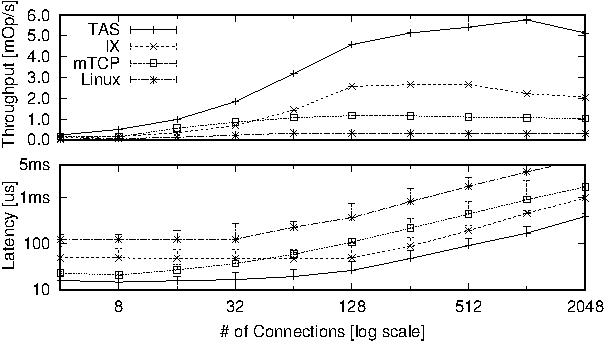
\includegraphics[width=\columnwidth]{plots/urpc/urpc.pdf}
  \caption{RPC echo throughput and latency (median and 99th percentile) for a
  single-threaded server.}
  \label{fig:tcpecho_combined}
\end{figure}

% 4  conn: TAS = 0.235122 linux = 0.036660, mtcp = 0.169545, IX = 0.0826
% 2k conn: TAS = 5.133833, linux = 0.305567, mtcp = 1.022676, IX = 2.05
\autoref{fig:tcpecho_combined} shows throughput as we vary the number
of client connections. With 4 connections \softtcp shows a throughput
of 6.4$\times$ Linux, 1.4$\times$ mTCP, and 2.8$\times$ IX. The
improvement is because \softtcp streamlines processing and thus gains
efficiency. mTCP comes closest but does not provide protection. All
stacks except Linux then scale until saturation. \softtcp's division
of labor into common and uncommon TCP processing experiences less
contention on uncommon data structures, resulting in improved
throughput. At 2,048 connections, \softtcp shows throughput of
16.8$\times$ Linux, 2.5$\times$ IX, and 5$\times$ mTCP. IX scales
better than mTCP, but not as well as \taas. This is because IX starts
to batch packets at 128 connections (average batch size 9 packets),
which gives it a throughput boost versus mTCP, but leads to increasing
per-packet latency. IX can maintain high throughput until 512
connections (average batch size 64 packets, which is the default
maximum). Starting with 1,024 simultaneous connections, IX starts to
drop an increasing number of packets that it cannot process, leading
to decreasing throughput. A similar effect happens for \taas, but
\taas has lower per-packet processing latency, leading to higher
throughput.

% 4  conn: TAS = 16, linux = 120, mtcp = 23, IX = 49
% 2k conn: TAS = 388, linux = 6760, mtcp = 1685, IX = 960
\autoref{fig:tcpecho_combined} also shows RPC round-trip time (RTT) as
we increase the number of client connections. We can see that \softtcp
achieves 31\%, 67\%, and 87\% better median latency with 4 connections
than mTCP, IX, and Linux, respectively. As we increase the number of
concurrent connections, latency increases for all configurations, but
more slowly for \softtcp. At 2,048 concurrent connections, \taas
achieves 77\%, 60\%, and 94\% better median latency than mTCP, IX, and
Linux, respectively. Again, this is expected due to \rmttcp's
streamlining. Linux does not perform well in the tail, while mTCP and
IX perform roughly equivalent to the median until 128 connections,
after which queues start to build. The division of labor in \softtcp
provides lower tail latency, the 99th percentile is 0.4ms for \softtcp versus
4.9ms, 1.1ms, and 8.4ms for mTCP, IX, and Linux, respectively.

\paragraph{Pipelined RPC.} In cases without dependencies, RPCs can be
pipelined on a single connection. These transfers can still be limited
by TCP stack overheads, depending on RPC size. We compare pipelined
RPC throughput for different sizes by running a single-threaded
event-based server processing RPCs on 100 connections, partitioned
equally over 4 client machines using 4 threads each.  After each RPC
the server waits for an artificial delay of 250 or 1000 cycles to
simulate application processing. To break out improvements in receive
and transmission overhead, we run separate benchmarks, one where the
server only receives RPCs and one where it only sends.
% For \rmttcp, we evaluate both a POSIX
% sockets compatible version (\rmttcp SO) and one using our low-level
% API (\rmttcp LL).

\begin{figure}
  \centering
  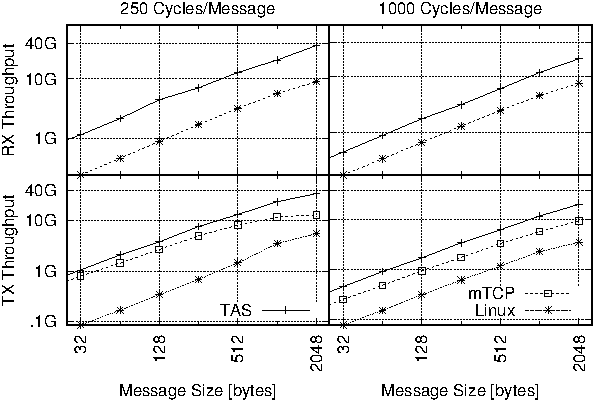
\includegraphics[width=\columnwidth]{plots/unidir/unidir}
  \caption{Pipelined RPC throughput, varying per-RPC delay and
    size, for a single-threaded server.}
  \label{fig:microunidir}
\end{figure}

% RX 64B 250c: TAS = 270483246  linux = 58013325
% RX 2K 250c: TAS = 4544184008  linux = 1128718921
\autoref{fig:microunidir} shows the results. When receiving small
($\leq$ 64B) RPCs, \rmttcp provides up to 4.5$\times$ better
throughput than Linux. \rmttcp's improvement reduces to 4$\times$ as
RPCs become larger. \rmttcp reaches 40G line-rate with 2KB RPCs for
250 cycles of processing while Linux barely reaches 10G. For 1000
cycles of processing, no stack achieves line-rate and \rmttcp provides
a steady throughput improvement around 2.5$\times$ regardless of RPC
size. % \antoine{The receive numbers are
  % potentially even a bit in Linux's favor because Linux uses RSS and
  % might process connections on multiple cores}.
%\softtcp's efficiency is between Linux and \rmttcp, which is
%expected given that it requires an additional host core to run the
%stack.
mTCP locks up in this experiment.

% TX 64B 250c: TAS = 264230525  linux = 21261640   mtcp = 181437669
% TX 2K 250c: TAS = 4293712283  linux = 698261349  mtcp = 1638577997
When sending small and moderate ($\leq$ 256B) RPCs at 250 cycles
processing time, \rmttcp provides up to 12.4$\times$ Linux and
1.5$\times$ mTCP efficiency. For large (2KB) RPCs, \rmttcp's advantage
declines to 6.1$\times$ Linux, but improves to 2.6$\times$ mTCP. mTCP
reaches scalability limitations beyond 512B RPCs, while Linux catches
up as memory copying costs start to dominate. \rmttcp again achieves
40G line-rate at 2KB RPC size, while Linux and mTCP do not reach
beyond 10G. This shows that simplifications in common-case send
processing, such as removing intermediate send queueing, can make a big
difference.

This difference again diminishes as application-level processing grows
to 1000 cycles. In this case, \rmttcp provides a steady improvement of
up to 5--6$\times$ Linux, regardless of RPC size. Compared to mTCP, \rmttcp
provides up to 2$\times$ improvement. \softtcp performs comparably to
mTCP in both transmit cases, but does provide protection.

\vspace{1ex}
\noindent We conclude that \rmttcp indeed provides better RPC latency
and throughput when compared to both state-of-the-art in-kernel and
kernel-bypass TCP stack solutions.
Further, \softtcp provides throughput on par with and better latency than
kernel-bypass stacks while retaining traditional OS safety guarantees.
Thus we improve performance and efficiency of all networked data center
applications relying on RPCs over TCP.

\subsection{Packet loss}

Even in a data center environment, minimal ($\leq$1\%) packet loss can
occur due to congestion and transmission errors. \rmttcp uses a
simplified recovery mechanism and we are interested how packet loss
affects \rmttcp throughput in comparison to Linux. We quantify this
effect in an experiment measuring throughput of 100 flows over a
single link between two machines under different rates of induced
packet loss between 0.1\% and 5\%. We compare \rmttcp with receiver
out-of-order processing and without it (simple go-back-N).
% also include simplified
% recovery for \rmttcp without the interval of out-of-order data at the
% receiver (basic go-back-N).

\begin{figure}
  \centering
  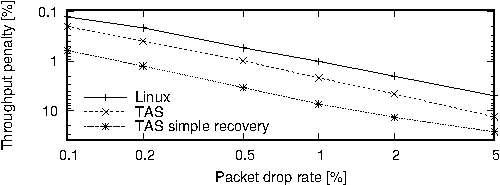
\includegraphics[width=\columnwidth]{plots/drops/throughput.pdf}
  \caption{Throughput penalty with varying packet loss rate.}
  \label{fig:packetdrops}
\end{figure}

\autoref{fig:packetdrops} shows the penalty relative to the throughput
achieved without loss. We can see that \rmttcp throughput is minimally
affected (up to 1.5\%) for loss rates up to 1\%. For a loss rate of
5\%, \rmttcp incurs a throughput penalty of 13\%. Overall, \rmttcp's
penalty is about 2$\times$ that of Linux. Linux keeps all received
out-of-order segments and also issues selective acknowledgements,
allowing it to recover more quickly. \rmttcp only keeps one continuous
interval of out-of-order data, requiring the sender to resend more in
some cases.  Without receiver out-of-order processing, the penalty
increases by a factor of 3. We conclude that limited out-of-order
processing has a benefit, but full out-of-order processing has minimal
impact for the loss rates common in data centers.

\subsection{Key-Value Store}\label{sec:kvstore}

Key-value stores strongly rely on RPCs. Due to the high TCP
processing overhead, some cloud operators use UDP for reads
and use TCP only for writing. % They then use application-layer
% mechanisms to combat the effect of packet loss or out-of-order
% arrival. TCP is typically used only to store values in the cache due
% to its reliability properties.
In this section, we demonstrate that \softtcp is fast enough to be used
for both reading and writing, simplifying application
design. To do so, we evaluate an optimized key-value store modeled
after memcached~\cite{memcached}. We send it requests at a constant
rate using a tool similar to the popular memslap benchmark. The
workload consists of 100,000 key-value pairs of 32 byte keys and 64
byte values, with a skewed access distribution (zipf, s = 0.9). The
workload contains 90\% GET requests and 10\% SET requests. Throughput
was measured over 2 minutes after 1 minute of warm-up.

\begin{figure}
  \centering
  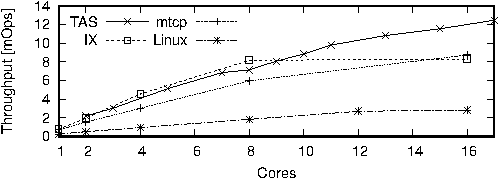
\includegraphics[width=\columnwidth]{plots/kvs/kvs.pdf}
  \caption{Key-value store throughput scalability.}
  \label{fig:memcached}
\end{figure}

\begin{table}
  \small
  \centering
  \begin{tabular}{lrrrr}
    \toprule
    \textbf{Latency [$\mu$s]} & \textbf{Median} & \textbf{90th} & \textbf{99th} & \textbf{99.9th} \\
    \midrule
    Linux & 124 & 153 & 200 & 275 \\
    mTCP & 28 & 33 & 40 & 71 \\
    IX & 49 & 53 & 70 & 83 \\
    \softtcp & 17 & 19 & 22 & 38 \\
    \bottomrule
  \end{tabular}
  \caption{Key-value store request latency in microseconds.}
  \label{tab:memcached_latency}
\end{table}

% 2C:  tas = 2.20  linux = 0.51 (4.3x)  mtcp = 1.54 (1.42x)  ix = 1.97 (1.12x)
% 16C: tas = 12.0  linux = 2.81 (4.27x) mtcp = 8.74 (1.37x)  ix = 8.29 (1.45x)
\paragraph{Throughput scalability.} To conduct throughput benchmarks
we run 4 clients, each using 4 cores to generate requests directed at the
server.
We establish between 128 and 2048 connections, chosen so as to maximize
throughput for each data point.
We run the
benchmark, varying the number of server application cores
available. Figure~\ref{fig:memcached} shows the result, counting all
host cores in use for the application and \rmttcp. We can see that
\rmttcp outperforms Linux, mTCP, and IX in total throughput by up to
4.3$\times$, 1.4$\times$, and 1.5$\times$, respectively.

\paragraph{Latency.} We also conduct single-core latency experiments
under 15\% bandwidth utilization, so that queues do not build
excessively. Table~\ref{tab:memcached_latency} show the result.
We can see that \rmttcp outperforms Linux, mTCP, and IX
by a median 7.3$\times$, 1.6$\times$, and 2.9$\times$, respectively.
\rmttcp also attains similar improvements in tail latency versus Linux, mTCP,
and IX.

\vspace{1ex}
\noindent We conclude that \rmttcp can greatly improve the performance
of RPC-based client-server applications, such as key-value stores. It
exceeds state-of-the-art network stacks in both latency and throughput
by a comfortable margin, both in median and the tail. As such, \rmttcp
can simplify the design of RPC-based applications by allowing them 
to rely on TCP instead of application-level solutions.

\subsection{Real-time Analytics}

Real-time analytics platforms are useful tools to gain instantaneous,
dynamic insight into vast datasets that change frequently. These
systems must be able to produce answers within a short timespan and
process millions of dataset changes per second. To do so, analytics
platforms utilize data stream processing techniques: A set of
\emph{workers} run continuously on a cluster of machines; data
\emph{tuples} containing updates stream through them according to a
dataflow processing graph, known as a \emph{topology}.
%
% Tuples are emitted and consumed worker-to-worker. Each worker can
% process and aggregate incoming tuples before emitting new tuples. 
The system scales by replicating workers over multiple cores and spreading incoming tuples
over the replicas. % This allows workers to process the data set in
% parallel. 
To minimize loss, many implementations transmit tuples via the TCP protocol.

To direct tuples to worker cores on each machine, a demultiplexer
thread is introduced that receives all incoming tuples and forwards
them to the correct executor for processing. Similarly, outgoing
tuples are first relayed to a multiplexer thread that batches tuples
before sending them onto their destination connections for better
performance.

% A typical example application for real-time analytics is determining
% the top-$n$ most active users of an interactive system. For example,
% the top-$n$ tweeting users of Twitter. To do so, tweets are injected
% as tuples into a set of counting workers to extract and then count the
% user name field within each tuple. The rest of the tuple is
% discarded. Periodically, counters emit a tuple for each active user
% name together with its count to a number of rankers. Rankers sort
% incoming tuples by count and emit the top-$n$ counted users to a
% single aggregating ranker. The aggregator produces the final output
% rank to the user.

\paragraph{Testbed setup.} We evaluate the performance of the \mystorm
real-time analytics platform, obtained from the authors of
\cite{flexnic}, by running the same
benchmark presented in \cite{flexnic}. % Our input workload is a
% stream of 476 million Twitter tweets collected between June--Dec 2009
% \cite{snapnets}. This setup is identical to the one used in
% \cite{flexnic}. 
Figure~\ref{fig:mystorm_throughput} and Table~\ref{tbl:mystorm_cycles}
show average achievable throughput and latency at peak load on this
workload. Throughput is measured over a runtime of 20 seconds, shown
raw and per core over the entire deployment. Per-tuple latency is
broken down into time spent in processing, and in input and output
queues, as measured at user-level, within \mystorm. We deploy \mystorm
on 3 machines of our client cluster. We evenly distribute workers
over the machines to balance the load.

\begin{figure}
  \centering
  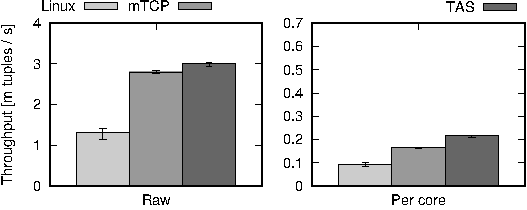
\includegraphics[width=\columnwidth]{plots/storm_tput/storm_tput_split.pdf}
  \caption{Average throughput on various \mystorm
    configurations. Error bars show min/max over 20 runs.}
  \label{fig:mystorm_throughput}
\end{figure}

\paragraph{Linux performance.} Overhead introduced by the Linux kernel
network stack limits \mystorm performance. Even though per-tuple
processing time is short, tuples spend several milliseconds in queues
after reception and before emission. Queueing before emission is due
to batching in the multiplexing thread, which batches up to 10
milliseconds of tuples before emission. Input queueing is minimal in
\mystorm as it is past the bottleneck of the Linux kernel and thus
packets are queued at a lower rate than they are removed.

% \paragraph{mTCP implementation.} In order to execute \mystorm with
% mTCP, we dedicate an additional core to execute the mTCP network stack
% and run \mystorm on the remaining cores. This was the highest
% performing configuration for \mystorm on mTCP. We could not run a
% per-core mTCP thread, as mTCP runs isolated network stack instances on
% each thread, relying on the NIC's RSS hash to distribute packets to
% each instance to scale to many cores. This does not work for
% asymmetric applications, like \mystorm, where the sets of receiving
% and sending threads are disjoint. A packet might be assigned via RSS
% to a thread that is not programmed to receive and will thus be
% discarded.

\paragraph{mTCP performance.} Running all \mystorm nodes on mTCP
yields a 2.1$\times$ raw throughput improvement versus Linux, while
utilizing an additional core per node to execute the mTCP user-level
network stack. The per-core throughput improvement is thus lower,
1.8$\times$. We could not run mTCP threads on application cores, as mTCP relies
on the NIC's symmetric RSS hash to distribute packets to isolated
per-thread stacks for scalability. This does not work for asymmetric
applications, like \mystorm, where the sets of receiving and sending
threads are disjoint. The bottleneck is now the \mystorm multiplexer
thread. Input queuing delay has increased dramatically, while output
queueing delay decreased only slightly. This is primarily because mTCP
collects packets into large batches to minimize context switches among
threads. Overall, tuple processing latency has decreased only 10\%
versus Linux due to the much higher amount of batching in mTCP.

\paragraph{\rmttcp performance.} Running all \mystorm nodes on \rmttcp
yields an 8\% raw throughput improvement versus mTCP and the per-core
throughput improvement is 26\%. The improvement is only small as the
bottleneck remains the multiplexer thread. Overall, tuple processing
latency has decreased 56\% versus mTCP. This is because \rmttcp does
not require any batching to achieve its performance.

% \paragraph{Object steering.} Enhancing \mystorm on \rmttcp with object
% steering support yields a 1.6$\times$ raw throughput improvement
% versus the non-steering version. Object steering has eliminated the
% multiplexer and demultiplexer threads on each node. Due to the
% elimination of their queues, tuple processing latency has decreased by
% 4 orders of magnitude versus not steering, while per-core throughput
% has improved by 2.8$\times$. The busiest workers in the system now
% operate at 90\% CPU utilization. Throughput is 13\% lower than the
% DCCP-based version of \mystorm~\cite{flexnic}. The difference is due
% to TCP's longer protocol header and congestion control mechanism (DCCP
% only supports flow control). To support object steering, we had to
% modify the processing loop of \mystorm's worker threads to use
% \rmttcp's object API and eliminate the (de-)multiplexing threads. This
% entailed changing roughly 20 lines of code (LOC) and removing hundreds
% of LOC.

\begin{table}
  \small
  \centering
  \begin{tabular}{lrrrr}
    \toprule
    & Input & Processing & Output & \textbf{Total}\\
    \midrule
    Linux & 6.96 $\mu$s & 0.37 $\mu$s & 20 ms & \textbf{20 ms} \\
    mTCP & 4 ms & 0.33 $\mu$s & 14 ms & \textbf{18 ms} \\
    \rmttcp & 7.47 $\mu$s & 0.36 $\mu$s & 8 ms & \textbf{8 ms} \\
    % Steering & -- & 0.30 $\mu$s & -- & \textbf{0.30 $\mu$s} \\
    \bottomrule
  \end{tabular}
  \caption{Average \mystorm tuple processing time.}
  \label{tbl:mystorm_cycles}
\end{table}

\vspace{1ex}
\noindent While there are limited throughput improvements to using
\taas due to application-level bottlenecks, we conclude that tuple
processing latency can be improved tremendously compared to approaches
that use batching, as fewer tuples are held in queues. This provides
the opportunity for tighter real-time processing guarantees under
higher workloads using the same equipment.

% We can use these results to predict what would happen at higher
% line-rates. The performance difference of roughly 2$\times$ between
% \flexnic and a fast software implementation shows that we would
% require at least 2 fully utilized hyperthreads to perform
% demultiplexing for \mystorm at a line-rate of 10Gb/s. As line-rate
% increases, this number increases proportionally, taking away threads
% that could otherwise be used to perform more analytics.

\subsection{Congestion Control}

We implemented DCTCP congestion control in \rmttcp with the key
difference that transmission is rate based, with rates updated
periodically for all flows by the kernel at a fixed pre-defined
control interval $\tau$. We investigate the impact of $\tau$ on
congestion behavior via ns-3 simulations, comparing to vanilla
DCTCP. First, we simulate a single 10Gbps link with an RTT of
100\textmu s at 75\% utilization with Pareto-distributed flow sizes
and varying $\tau$. Next, we simulate a large cluster of 2560 servers
and a total of 112 switches that are configured in a 3-level FatTree
topology with an oversubscription ratio of 1:4.
% The core and aggregation switches each have $16 \times 10$Gbps ports
% while the ToRs each have $4 \times 10$Gbps ports and $40 \times 1$Gbps
% ports.
All servers follow and on-off traffic pattern, sending flows to a
random server in the data center at a rate such that the core link
utilization is approximately 30\%. Finally, we investigate congestion
fairness experimentally with $\tau = 2\times\mathrm{RTT}$ (as measured for each
flow) under incast.

\paragraph{Single link.} Figure~\ref{fig:ns3-link} shows average flow
completion time (FCT) and average queue size with varying $\tau$ for
the single 10Gbps link. The average FCT for \rmttcp is very similar to
that of DCTCP when $\tau$ is greater than the RTT. However, if $\tau$
is set too low, frequent fluctuations in congestion window cause slow
convergence and long completion times. The average queue length is
very similar to that of DCTCP and grows, but slowly, as $\tau$
increases beyond the RTT, due to delayed congestion window updates.

\begin{figure}
  \vspace{-1.8ex}
  \centering
  \subfloat[Avg flow completion time]{%
    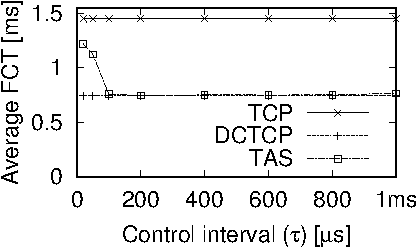
\includegraphics[width=0.5\columnwidth]{plots/ns3/fct-link.pdf}
  }\hspace*{-0.25cm}
  \subfloat[Average queue length]{%
    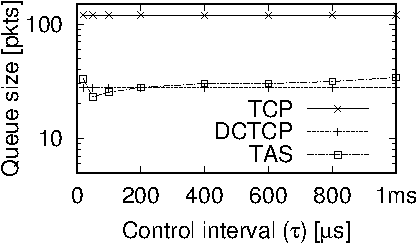
\includegraphics[width=0.5\columnwidth]{plots/ns3/queue-link.pdf}
  }
  \caption{Simulation of a single 10Gbps link.}
  \label{fig:ns3-link}
\end{figure}

\paragraph{Large cluster.} Figure~\ref{fig:ns3-cluster} shows the
average flow completion times for short and long flow sizes in the
large cluster simulation with the control interval $\tau$ set to
100\textmu s. The performance of \rmttcp is similar to that of DCTCP
in both cases. 100\textmu s is a reasonable amount of time for the
kernel to update congestion windows for thousands of flows. Even with
larger values of $\tau$, queue size is only minimally affected and
FCTs stay approximately identical. We thus conclude that our
out-of-band approach works to provide DCTCP-compatible congestion
behavior.

%  {\it Should we
% comment on the fact that it's reasonable to set $tau$ to 100\textmu s?
% It's not too low and the kernel thread can update all congestion windows
% in this time.}

\begin{figure}
  \vspace{-1.8ex}
  \centering
  \subfloat[Short flows $\leq$ 50 pkts]{%
    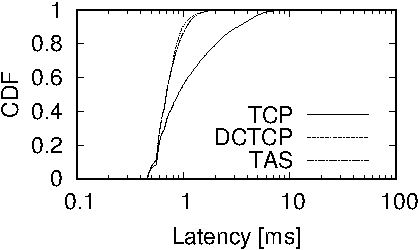
\includegraphics[width=0.5\columnwidth]{plots/ns3/fct-short-cluster.pdf}
  }\hspace*{-0.25cm}
  \subfloat[Long flows $>$ 50 pkts]{%
    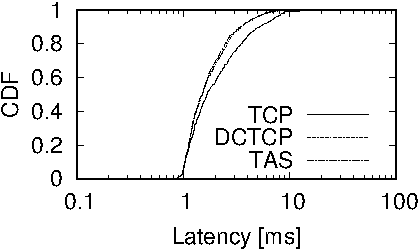
\includegraphics[width=0.5\columnwidth]{plots/ns3/fct-long-cluster.pdf}
  }
  \caption{Flow completion times for large cluster simulation.}
  \label{fig:ns3-cluster}
\end{figure}

% {\it We can also cite this paper from NSDI-17, (Flowtune: Flowlet Control
% for Datacenter Networks), in which CC decisions are made at flowlet
% granularity, because it avoids packet-level rate fluctuations that leads
% to fast convergence.}
%

\paragraph{Tail-latency under incast.} To evaluate performance under
congestion, we measure tail latency under incast with 4 machines
sending to a single receiver (operating at line rate) with different
numbers of connections.  We record the number of bytes received on
each connection every 100ms on the receiver over the period of a
minute, discarding a warmup 20 seconds.  \autoref{fig:fairness} shows
the median (and 99th percentile) throughput over the measured
intervals and connections on Linux (using DCTCP) and \rmttcp.  For
\rmttcp, the tail falls within $1.6\times$ and $2.8\times$ of the
median, while the median is close to each connection's fair
share. Linux median (and tail---not shown) behavior fluctuates
widely, showing significant starvation of flows in some cases.

\begin{figure}
  \centering
  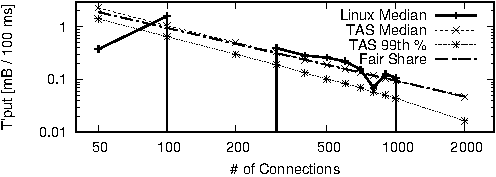
\includegraphics[width=\columnwidth]{plots/fairness_new/fairness.pdf}
  \caption{Distribution of connection rates under incast.}
  \label{fig:fairness}
\end{figure}

Linux fairness is hurt in three interacting ways: (1) Linux window
based congestion control creates bursts when windows abruptly widen
and contract under congestion. (2) Window-based congestion control
limits the control granularity for low-rtt links.  (3) The Linux TCP
stack architecture requires many shared queues that can overflow when
flows are bursty, resulting in dropped packets without regard to
fairness. Rate-based packet scheduling and per-flow queueing in
\rmttcp smoothes bursts and eliminates unfair packet drops at end
hosts.


\subsection{Workload Proportionality}
Finally, we analyze a dynamic workload to evaluate how \rmttcp adapts to
workload changes and how this affects end-to-end performance.
For this experiment, we re-use and instrument the key-value store server and
vary the number of clients over time.
At time 0 we start with one client machine, and add four additional client
machines, one every 10 seconds, after an additional 10 seconds we remove the
client machines again one by one.
\autoref{fig:autoscale_tp} shows both the number of fast-path cores for \rmttcp
as well as the total server throughput.
\rmttcp starts out with just 1 core, and ramps up to 3 cores for the first
client, and continues to add additional cores until reaching 9 cores, before
incrementally removing cores again as the load reduces.
\autoref{fig:autoscale_l} shows request latency as measured by clients as for
the transition from 3 to 4 clients and with it 7 to 9 cores.
During the adjustment the latency temporarily spikes by about $15\mu$s or 30\%
before quckly returning back to the previous level.
We conclude that \rmttcp is able to adapt to workload changes, acquiring and
releasing processors as needed, without significantly impacting end-to-end
latency or throughput.

\begin{figure}
  \centering
  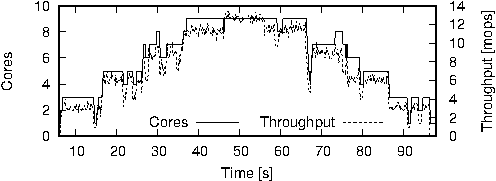
\includegraphics[width=\columnwidth]{plots/autoscale/autoscale}
  \caption{Number of \rmttcp processor cores and end-to-end throughput as
  key-value store server load first increases and then decreases again.}
  \label{fig:autoscale_tp}
\end{figure}

\begin{figure}
  \centering
  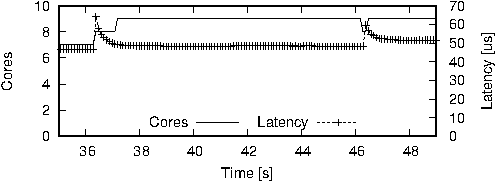
\includegraphics[width=\columnwidth]{plots/autoscale/autoscale_latency}
  \caption{End-to-end request latency as \rmttcp acquires additional processor
  cores in response to increasing load.}
  \label{fig:autoscale_l}
\end{figure}
